%%%%%%%%%%%%%%%%%%%%%%%%%%%%%%%%%%%%%%%%%%%%%%%%%%%%%%%%%%%%%%%
%
% Welcome to Overleaf --- just edit your LaTeX on the left,
% and we'll compile it for you on the right. If you open the
% 'Share' menu, you can invite other users to edit at the same
% time. See www.overleaf.com/learn for more info. Enjoy!
%
%%%%%%%%%%%%%%%%%%%%%%%%%%%%%%%%%%%%%%%%%%%%%%%%%%%%%%%%%%%%%%%


% Inbuilt themes in beamer
\documentclass{beamer}

% Theme choice:
\usetheme{CambridgeUS}

 \providecommand{\pr}[1]{\ensuremath{\Pr\left(#1\right)}}
 \providecommand{\sbrak}[1]{\ensuremath{{}\left[#1\right]}}
 \providecommand{\brak}[1]{\ensuremath{\left(#1\right)}}
 \providecommand{\cbrak}[1]{\ensuremath{\left\{#1\right\}}}

% Title page details: 
\title{Assignment 8} 
\author{Donal Loitam - AI21BTECH11009}
\date{\today}
\logo{\large \LaTeX{}}

\usepackage{hyperref}
\usepackage{mathtools}
\usepackage{amssymb}
\usepackage{amsmath}


\begin{document}

% Title page frame
\begin{frame}
    \titlepage 
\end{frame}

% Remove logo from the next slides
\logo{}


% Outline frame
\begin{frame}{Papoulis chap 4 Ex 4.8}
TABLE OF CONTENTS
    \tableofcontents
\end{frame}


% Lists frame
\section{Question}
\begin{frame}{Problem}
\textbf{Example 4-8:  }Suppose the random variable $X$ is such that   $X\brak{\xi} = 1$ if $\xi \in A$ and zero otherwise. Find $F(x)$
\end{frame}

\section{Solution}
\begin{frame}{Solution}
  Let $\pr{A} = p$, denote the probability of the event $A$ happening and '$S$' denote the universal set.\\
   Given, \[
        X\brak{\xi}=\left\{
                \begin{array}{ll}
                  1 \;\;\;\;\;\;\;\;\;    if \;\xi \in A \\
                  0  \;\;\;\;\;\;\;\;\;    else
                \end{array}
              \right.
  \]
  For $ x<0 $ , $\cbrak{X\brak{\xi} \le x} = \cbrak{\emptyset}$ , so that $F(x)=0$ \\
  For $ 0 \le x < 1 $, $\cbrak{X\brak{\xi} \le x} = \cbrak{A'}$, so 
that $F(x) = \pr{A'} = 1 - p = q $
For $ x \ge 1 $, $\cbrak{X\brak{\xi} \le x} = S$, so that $F(x) = 1$ (see figure).
\end{frame}

\begin{frame}{Solution(Contd.)}
Hnece, $F(x)$ can be written as :-
        \[
        F(x)=\left\{
                \begin{array}{ll}
                  0  \;\;\;\;\;\;\;\;\;\;\;\;\;\;\;\; \;\; \; , x \in \brak{-\infty,0}  \\
                  1-p  \;\;\;\;\;\;\;\;\;\;\;  \; \;, x \in [\; 0,1)  \\
                  1  \;\;\;\;\;\;\;\;\;\;\;\;\;\;\;\; \;\;\;  , x \in [\;1,\infty)
                  \end{array}
              \right.
       \]
       The corresponding graph of $F(x)$ is plotted next page :-
\end{frame}

\section{Graph}
\begin{frame}{CDF Graph}
    \begin{figure}[!ht]
		\centering
		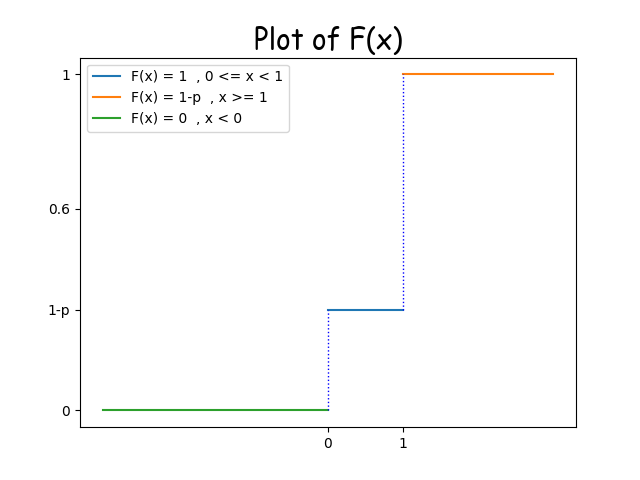
\includegraphics[width=\textwidth,height=6.2cm,keepaspectratio]{cdf_plot.png}
		\caption{CDF function}
		\label{fig1}
	\end{figure}
\end{frame}

% % Blocks frame
\section{Codes}
\begin{frame}{CODES}
    \begin{block}{Python}
         Download python code from - \href{https://github.com/Donal-08/Assignment_8/blob/main/code/cdf_plot.py}{Python}
    \end{block}

 \begin{block}{Beamer}
         Download Beamer code from - \href{https://github.com/jarpula-Bhanu/Assignment-8/blob/main/beamer_8.tex}{Beamer}
    \end{block}
\end{frame} 

\end{document}
